\documentclass[amsmath,amssymb, aps, prx, longbibliography, twocolumn]{revtex4-1}

\usepackage{natbib}
\usepackage{graphicx}% Include figure files
\usepackage{dcolumn}% Align table columns on decimal point
\usepackage{bm}
\usepackage[usenames]{color}
\usepackage{subfigure}

\newcommand{\cb}[1]{\textcolor{magenta}{[Carsten: #1]}}


\begin{document}

\title{ Detecting non-Fermi liquid transport in the quantum critical region \\ via quantum loop topography}

\author{George (Trey) Driskell$^1$}
\author{Samuel Lederer$^1$}
\author{Carsten Bauer$^2$}
\author{Simon Trebst$^2$}
\author{Eun-Ah Kim$^1$}
\email{eun-ah.kim@cornell.edu}

\affiliation{%
$^{1}$Department of Physics, Cornell University, Ithaca, New York 14853, USA}%
\affiliation{$^{2}$Institute for Theoretical Physics, University of Cologne, 50937 Cologne, Germany}

\date{\today}

\begin{abstract}
Anomalous transport, such as T-linear resistivity (a hallmark of non-Fermi liquid behavior), is a ubiquitous feature of strongly correlated metallic systems, but famously difficult to understand theoretically. For relevant simple models, the transport computations of even numerically exact Monte Carlo simulations are subject to enormous systematic errors and come at great additional computational cost. Building on earlier work, we apply quantum loop topography (QLT) and supervised learning on quantum Monte Carlo data to examine the Fermi liquid to non-Fermi liquid crossover in models of both Ising nematic and \cb{antiferromagnetic} spin density wave quantum criticality. Previous work on these models has demonstrated this crossover using measurements of correlation functions at nonzero imaginary time separation. Our results, using only equal time measurements, show good agreement with these previous results at dramatically lower computational cost. Hence, QLT-based machine learning can accelerate the exploration of parameter space in search for non-Fermi liquid behavior by obviating the need for expensive dynamical measurements.
\end{abstract}

\maketitle

%%%%%%%%%%%%%%%%%%%%%%%%%%%%%%%%%%%%%%%%%%%%%%%%%%%%%%%%%%%%%%%%%%
% Introduction
%%%%%%%%%%%%%%%%%%%%%%%%%%%%%%%%%%%%%%%%%%%%%%%%%%%%%%%%%%%%%%%%%%
[1 problem statement: NFL in QC -- Simon ]
Most often defined by transport in experiment, ubiquitous
\\
\\
\\
\\
\\
\\
\\
\\
\\
\\
\\


[2 literature in sign-free MC -- Simon]
Transport is hard. "proxies" are not satisfactory.
\\
\\
\\
\\
\\
\\
\\
\\
\\
\\
\\
\\
\\
\\
\\

[3 literature in phase recognition -- EK]
Ideal application of ML is where conventional approaches are lacking: such as topological order and NFL.
 \\
 \\
 \\
 \\
 \\
 \\
 \\
 \\
 \\
 \\
 \\
 \\
 \begin{figure} [t]
    \centering
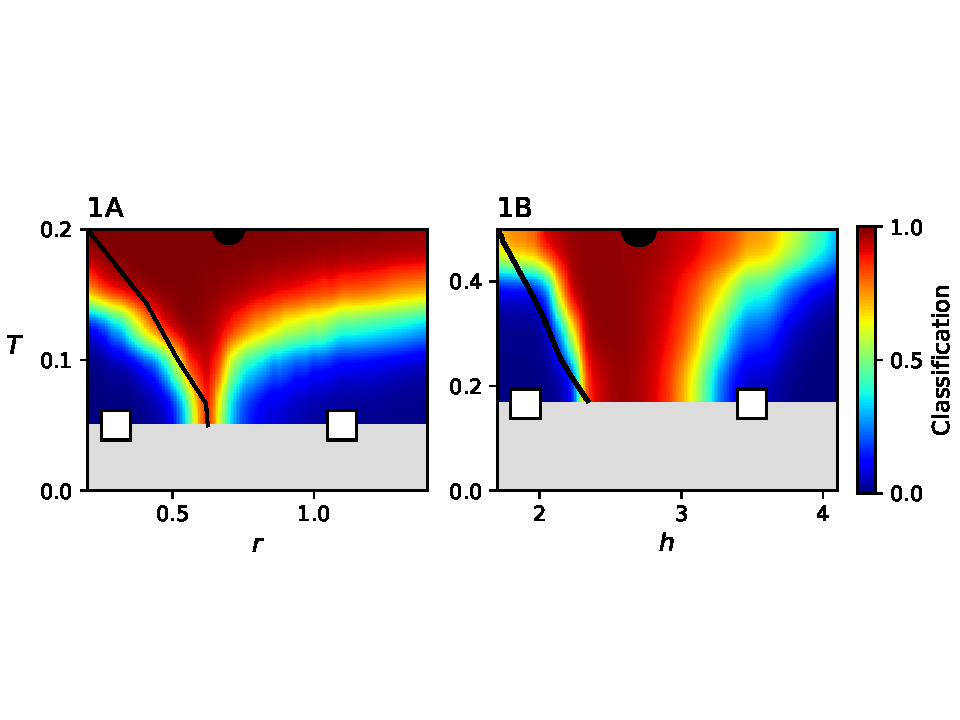
\includegraphics[width=.5\textwidth, trim={0 2.75cm 0 3cm}, clip]{3pt_pds.pdf}
    \caption{Phase diagrams of quantum critical metals overlaid with machine-learned Fermi liquid to non-Fermi liquid crossover. The color maps show the output of the neural networks trained to classify Fermi liquid and non-Fermi liquid regimes of the spin density wave model (1A, Eq. \ref{Eq:SDW}, with $\lambda =1.5,c=3,u=1,\mu=\textbf{what?}$) and the nematic model (1B, Eq. \ref{Eq:Nematic}, with $\alpha=1.5,V=0.5,\mu=-1$).
    A value of 1 (dark red) corresponds to the non-Fermi liquid, a value of 0 (dark blue) corresponds to the Fermi liquid, and intermediate values represent the crossover region. The neural networks are trained using Quantum Loop Topography data drawn from quantum Monte Carlo simulations of the models at the training points shown in the figure: white boxes for the Fermi liquid (1A: $r=0.3,T=0.05$ and $r=1.1,T=0.05$; 1B: $h=1.9,T=0.17$ and $h=3.5,T=0.17$) and black circles for the non-Fermi liquid (1A: $r=0.7,T=0.2$; 1B: $h=2.7,T=0.5$). The black lines show the phase boundaries, from refs \cite{Lederer4905,Gerlach2017}.}
    \label{fig:pds}
\end{figure}
[4 In this paper - Fig 1] 
\\
\\
\\
\\
\\
\\
\\
\\


[5 Two QCP's to study -- EK]
Their similarities and differences in words.
\\
\\
\\
\\
\\
\\
\\
\\
\\

 \begin{figure} [t]
    \centering
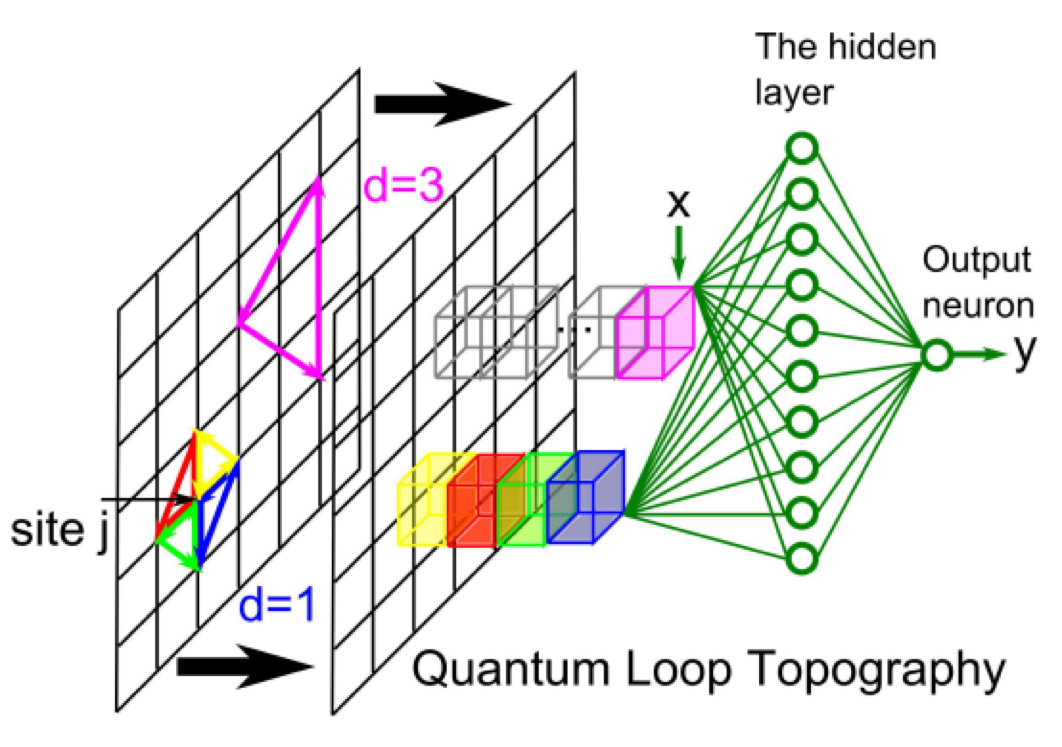
\includegraphics[width=.5\textwidth]{qlt.png}
    \caption{Caption}
    \label{fig:qlt}
\end{figure}
[6 ML architecture and preprocessing -- Trey FIG \ref{fig:qlt}]
Following previous efforts \cite{Zhang2019}, Quantum Loop Topography (QLT) was used to preprocess the training data, which consist of quantum Monte Carlo samples of the equal-time Green function at fixed points in parameter space (8000 samples for the nematic model and 4000 samples for the SDW model). QLT extracts from a given sample features equal to chained products of the equal-time Green function that form both triangular and quadrilateral loops on the lattice sites. We limit the length of the loops to only consider nearest neighbor and next-nearest neighbor sites for forming a chain in each loop. The QLT vectors are then standardized by subtracting the mean and dividing by the standard deviation of each feature evaluated over the entire training dataset. After the data are preprocessed, they are fed to a feed-forward fully-connected neural network with one hidden layer of $n=10$ sigmoid neurons. Prior to the output layer, batch normalization is performed on the hidden layer. The network is trained using stochastic gradient descent with a binary cross-entropy cost function, L2 regularization to avoid over-fitting, and a mini-batch size of 16. \\ 

[7 SDW model action and what is known -- Carsten]
As a first principle model, we consider a system of itinerant fermions coupled to antiferromagnetic spin-density wave order in which quantum critical fluctuations give rise to high-temperature superconductivity and lead to fermionic quasiparticle decoherence beyond the Fermi liquid paradigm \cite{Bauer2020, Schattner2016, Gerlach2017, Liu2018}.
Specifically, we focus our analysis on the sign-problem free \cite{Berg2012, Wu2005} two-dimensional spin-fermion model of Refs.~\cite{Schattner2016, Gerlach2017, Zhang2019}, which have determined the quantum critical properties in extensive, numerically exact DQMC studies. The action of the system is given by $S = S_\psi + S_\varphi + S_\lambda$,
\begin{eqnarray}
\label{Eq:SDW}
S_\psi &=&  - \int_{\tau, \mathbf{r}, \mathbf{r'}} \sum_{s, \alpha} \left[ \left(\partial_\tau - \mu\right)\delta_{\mathbf{r}\mathbf{r'}} - t_{\alpha \mathbf{r}\mathbf{r'}} \right] \psi_{\alpha \mathbf{r}s}^\dagger \psi_{\alpha \mathbf{r'}s} \nonumber\\
S_\varphi &=& \int_{\tau,\mathbf{r}} \frac{1}{2c^2} \left(\partial_\tau \vec{\varphi}\right)^2 + \left(\nabla \vec{\varphi} \right)^2 + \frac{r}{2}\vec \varphi^2 + \frac{u}{4} (\vec \varphi^2)^2 \label{eq:afmetal}\\
S_\lambda &=& \lambda \int_{\tau, \mathbf{r}} e^{i \mathbf{Q}\cdot \mathbf{r_i}} \vec{\varphi}_\mathbf{r} \cdot \left( \psi_{a\mathbf{r}s}^\dagger \vec{\sigma}_{ss'}  \psi_{b\mathbf{r}s'} + \textrm{h.c.} \right), \nonumber
\end{eqnarray}
where $\alpha=a,b$ is a fermion flavor index and $s=\uparrow, \downarrow$ denotes spin. $S_\psi$ describes the free kinetics of two flavors of spin-1/2 fermions $\psi_{\alpha \mathbf{r} s}$ situated on a square lattice. The antiferromagnetic order parameter $\varphi$ is of easy-plane character and is governed by a $O(2)$ symmetric $\varphi^4$-theory. The contribution $S_\lambda$ is a Yukawa-like spin-density coupling with an ordering wave vector $\mathbf{Q} = (\pi,\pi)$, which connects different scattering hot spots on the Fermi surface. All parameters are chosen as for Fig.~2b in Ref.~\cite{Gerlach2017}, namely $\lambda=1.5$, $c=3$ and $u=1$.

It is instructive to discuss the findings of Ref.~\cite{Gerlach2017}, as they will serve as an important guide and benchmark for our QLT analysis. The traditional method for locating the SDW phase transition of model~\eqref{eq:afmetal} is based on a finite-size scaling analysis of antiferromagnetic correlations: Given that the transition is of Berezinskii–Kosterlitz–Thouless type the phase boundary of the ordered state is characterized by the universal critical exponent $\eta = 1/4$. Tracing the transition down to $T=0$ one obtains an estimate for the QCP location of about $r_c = 0.62$ \cite{Gerlach2017}. In the vicinity of this QCP, at finite temperatures, the Matsubara self-energy at the hot spots is found to be finite and only weakly dependent on Matsubara frequency indicating a non-Fermi liquid state in which quasiparticles have lost their coherence \cite{Gerlach2017}. Specifically, the quasiparticle weight at the hot spots drops significantly in this quantum critical region of the phase diagram.\cb{Should we mention the computational cost of these calculations?}
\\
\\
\\
\\
\\
\\
\\
\\
\\

[8 2pt classification for ordered phase -- EK. FIG \ref{fig:2ptsdw}]
\\
\\
\\
\\
\\
\\
\\
\\
 \begin{figure} [t]
    \centering
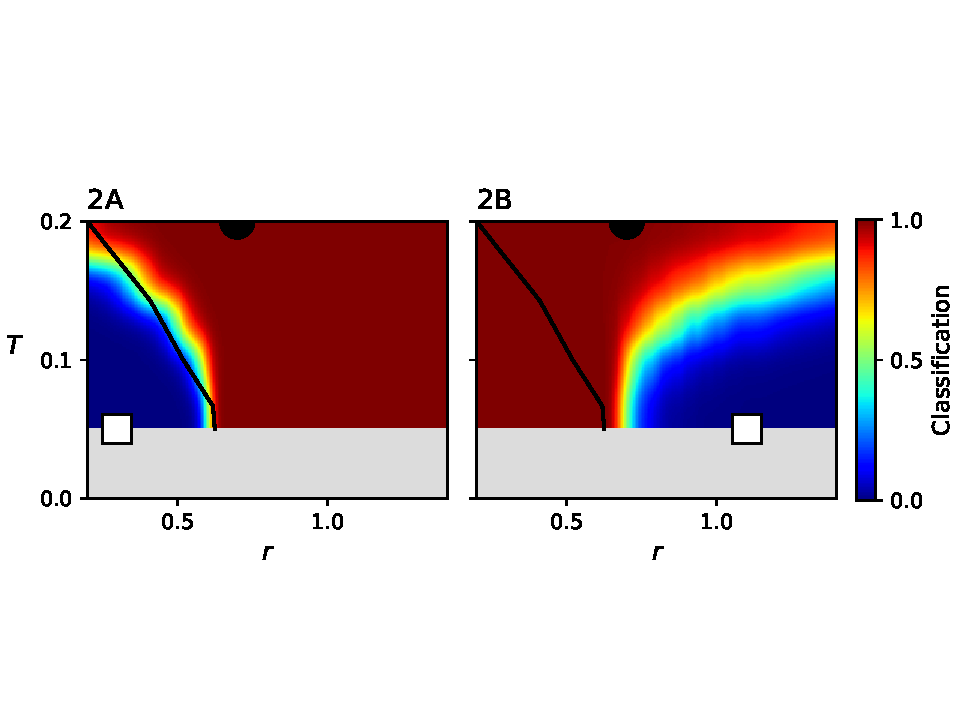
\includegraphics[width=.45\textwidth, trim={0 2.5cm 0 3cm}, clip]{2pt_sdw.pdf}
    \caption{Binary classification for the SDW model. (a) The neural network is trained to distinguish the quasi-long range ordered phase (training point at the white box, $r=0.3,T=0.05$) from the non-Fermi liquid regime (the black circle, $r=0.7,T=0.2$). (b) The neural network is trained to distinguish the disordered Fermi liquid regime (training point at the white box, $r=1.1,T=0.05$) from the non-Fermi liquid regime (the black circle, as in (a)).}
    \label{fig:2ptsdw}
\end{figure}

[9 2PT classification for NFL-FL and 3PT classification -- EK]
FIG \ref{fig:2ptsdw}, FIG \ref{fig:pds}
\\
\\
\\
\\
\\
\\
\\
\\




[10 Nematic action and what is known -- Sam]\\
Nematic quantum criticality has been extensively explored in Refs.~\cite{PhysRevX.6.031028,Lederer4905} on the basis of a lattice model. The model's degrees of freedom are spin 1/2 fermions $c_{i,\sigma}$ that live on the sites $i$ of a square lattice, and pseudospins $\tau_{i,j}$ that live on the nearest neighbor bonds $\left<i,j\right>$. The Hamiltonian is $H = H_{f} + H_{b} + H_{int}$, where:
\begin{align}
\label{Eq:Nematic}
    H_{f} &= -t\sum_{\left<i,j\right>,\sigma}c_{i\sigma}^{\dagger}c_{j\sigma}-\mu \sum_{i\sigma}c_{i\sigma}^{\dagger}c_{i\sigma} \nonumber \\
    H_{b} &= V \sum_{\left<\left<i,j\right>;\left<k,l\right>\right>}\tau^{z}_{i,j}\tau^{z}_{k,l}-h\sum_{\left<i,j\right>}\tau^{x}_{i,j}\\
    H_{int} &= \alpha t\sum_{\left<i,j\right>,\sigma}\tau^{z}_{i,j}c_{i\sigma}^{\dagger}c_{j\sigma} \nonumber
\end{align}
The nested brackets in the first term of $H_{b}$ represent nearest neighbor bonds. The ordered phase has pseudospins develop unequal expectation values on horizontal and vertical bonds, leading to an effective anisotropic hopping of the fermions.  
 
For sufficiently strong coupling $\alpha$, this model exhibits high temperature superconductivity with a maximum in the critical temperature $T_{c}$ near $h_{c} = 2.6$, the approximate position of the quantum critical point. For $h$ near $h_{c}$, and in a range of temperature above $T_{c}$, the fermion self-energy exhibits a strongly non-Fermi liquid dependence on Matsubara frequency, as well as transport signatures consistent with bad metallic behavior (though the challenges of analytic continuation prevent any definitive classification). By contrast, for larger $h$ and at sufficiently low temperature, the system's behavior is consistent with Fermi liquid theory.
% \begin{align*}
%     H &= H_{f} + H_{b} + H_{int} \\
%     H_{f} &= -t\sum_{\left<i,j\right>,\sigma}c_{i\sigma}^{\dagger}c_{j\sigma}-\mu \sum_{i\sigma}c_{i\sigma}^{\dagger}c_{i\sigma} \\
%     H_{b} &= V \sum_{\left<\left<i,j\right>;\left<k,l\right>\right>}\tau^{z}_{i,j}\tau^{z}_{k,l}-h\sum_{\left<i,j\right>}\tau^{x}_{i,j}\\
%     H_{int} &= \alpha t\sum_{\left<i,j\right>,\sigma}\tau^{z}_{i,j}c_{i\sigma}^{\dagger}c_{j\sigma}
% \end{align*}
\\
\\
\\
\\
\\
\\
\\
\\
\\

\begin{figure} [t]
    \centering
    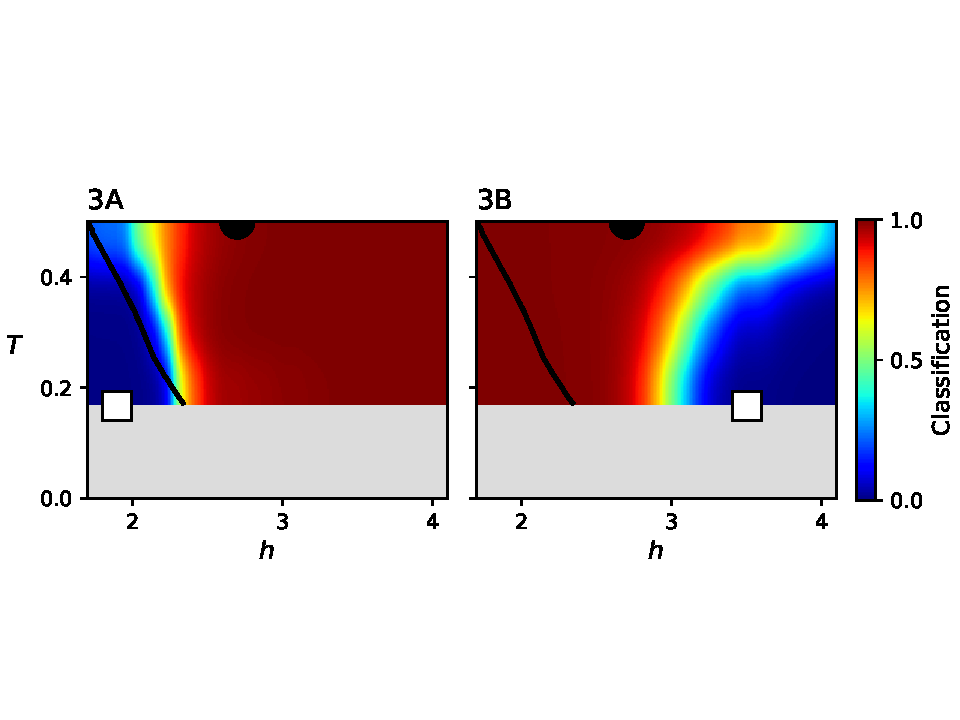
\includegraphics[width=.45\textwidth, trim={0 2.5cm 0 3cm}, clip]{2pt_nematic.pdf}
    \caption{Binary classification for the Nematic model. (a) The neural network is trained to distinguish the long range ordered phase (training point at the white box, $h=1.9,T=0.17$) from the non-Fermi liquid regime (the black circle, $h=2.7,T=0.5$). (b) The neural network is trained to distinguish the disordered Fermi liquid regime (training point at the white box, $h=3.5,T=0.17$) from the non-Fermi liquid regime (the black circle, as in (a)).}
    \label{fig:2ptnem}
\end{figure}

[11 2PT classification for ordered phase -- EK]
FIG \ref{fig:2ptnem}
\\
\\
\\
\\
\\
\\
\\
\\
\\
\\


[12 2PT classification for NFL-FL and 3pt classification --EK]
FIG \ref{fig:2ptnem}, FIG \ref{fig:pds}.
\\
\\
\\
\\
\\
\\
\\
\\
\\

[13 Summary --EK]

[14 Implications and Outlook --EK]



{\it Acknowledgements.--} 
We acknowledge useful discussions with XXX. SL and E-AK acknowledge the support from the U.S. Department of Energy, Office of Basic Energy Sciences, Division of Materials Science and Engineering under Award DE-SC0018946.
The Cologne group acknowledges partial support from the Deutsche Forschungsgemeinschaft (DFG, German Research Foundation) -- Projektnummer 277101999 -- TRR 183 (project B01).
The numerical simulations were performed on the JUWELS cluster at FZ J\"ulich and the CHEOPS cluster at RRZK Cologne.


%\bibliographystyle{apsrev4-1}
\bibliography{refs}
\appendix



\end{document}
